\documentclass[]{article}
\usepackage{graphicx}
\usepackage{subcaption}
\usepackage{amsmath}
\usepackage{amsfonts}
\usepackage{tikz}
\usepackage{hyperref}       % hyperlinks
\usepackage{url}            % simple URL typesetting
\newcommand{\argmax}{\operatornamewithlimits{argmax}}
\newcommand{\argmin}{\operatornamewithlimits{argmin}}




\tikzstyle{mybox} = [draw=black, fill=white,  thick,
rectangle, inner sep=10pt, inner ysep=20pt]
%opening


\begin{document}
%	\maketitle
	\noindent
%	\textbf{Definition} We call a matrix $A\in m\times n$ is $non-negative \;over \;complete(NN overcomplete)$ if $conv(A_i)$ where $A_i$ is a column of $A$, has $K$ vertices where $K \ll n$. 
\section{Computational results}
	\subsection{Synthetic data}
	\subsubsection{Feasibility problem}
	
	  
	In this section, we present experimental results which empirically show when the problem is 'over complete', \textbf{AVTA} can be a 'shortcut' solution. In another word, given an $m\times n$ matrix $A$ as data, where the convex hull of the columns of $A$, denoted by $conv(A)$, has $K$ vertices, $K \ll n$.  Let $\overline A$ denote the vertices of $conv(A)$. In some applications one simply needs to compute $\overline A$.  In many other applications the computation of $\overline A$ reduces the problem over $A$ to an equivalent problem over $\overline A$. Thus the complexity of solving a particular problem $\cal{P}$ on input $A$, denoted by $T({\cal{P}}(A))$, can alternatively be replaced with $T(\overline A)+ T({\cal{P}}(\overline A))$, where $T(\overline A)$ is the complexity of computing $\overline A$. We apply the \textbf{AVTA} to solve $2$ classical problems which appear in many applications. 
	%In all experiments, data are generated randomly and the computation is repeated for 10 times.  
	
	
	
	\noindent \textbf{Convex hull membership problem}: 
	The convex hull membership problem is to test if a given $p \in \mathbb{R}^m$ lies in $conv(S)$. The problem can be solved by \textbf{Triangle Algorithm} ~\cite{kalantari2015characterization} and \textbf{Frank Wolfe} ~\cite{jaggi2013revisiting} by producing an approximate solution $p_\epsilon$ where $d(p,p_\epsilon)  \leq \epsilon$. This problem can also solved by following linear program:\\
	\begin{equation}
		\begin{aligned}
		&min \;\;\; \vec{1} \cdot y\\
		&  A\alpha+\beta=p\\ 
		&  \sum_{i=1}^{K} \alpha_i=1\\
		& \alpha\geq0\;\;,\;\beta\geq0
		\end{aligned}
	\end{equation}
	where $p \in conv(s)$ if and only if the optimal solution of this linear program is $y^*=0$. In case when the number of vertices is much less than the number of points i.e. $n \gg K$, the membership problem can be reduced to following query: Is there exists $d+1$ vertices s.t. $p$ is $\epsilon$ close to the convex hull of these $d+1$ vertices? Since the \textbf{AVTA} can detect vertices progressively, it can be used to solve the membership query:
	\begin{center}
		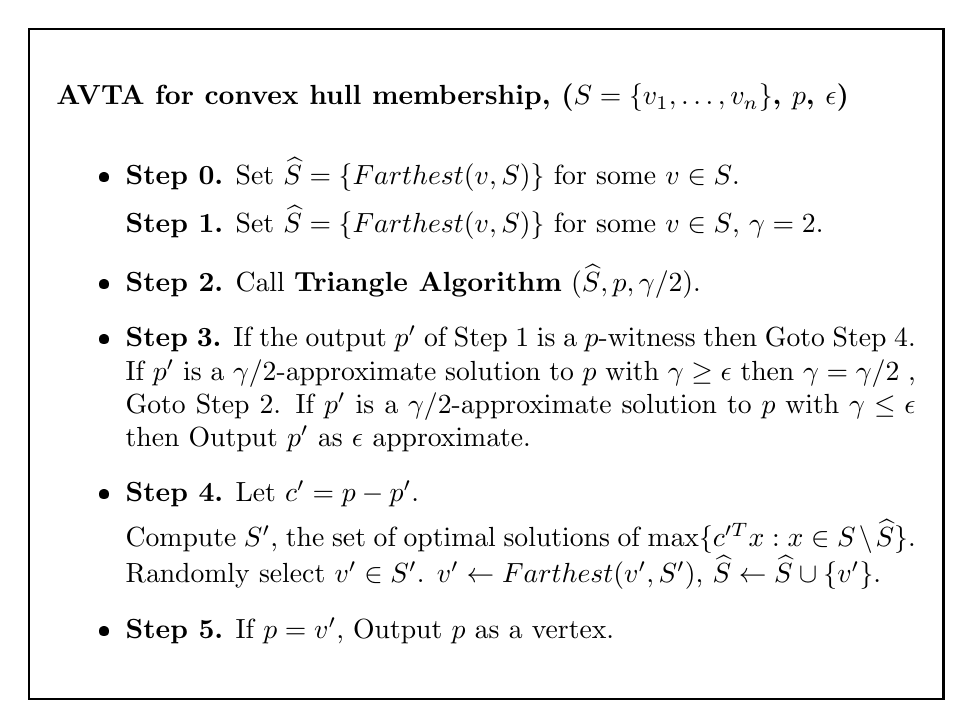
\begin{tikzpicture}
		%\begin{center}
		\node [mybox] (box){%
			\begin{minipage}{0.9\textwidth}
			{\bf AVTA for convex hull membership, ($S=\{v_1, \dots, v_n\}$, $p$, $\epsilon$)}\
			
			\vspace{.2cm}
			\begin{itemize}
			\item
			
			{\bf Step 0.} Set $\widehat S = \{Farthest(v, S)\}$ for some $v \in S$. 
			
			{\bf Step 1.} Set $\widehat S = \{Farthest(v, S)\}$ for some $v \in S$, $\gamma=2$. 			
			\item
			{\bf Step 2.} Call {\bf Triangle Algorithm} $(\widehat S, p,  \gamma/2)$.
			
			\item
			{\bf Step 3.}
			If the output $p'$ of Step 1 is a $p$-witness then Goto Step 4. If $p'$ is a $\gamma/2$-approximate solution to $p$ with $\gamma \geq \epsilon$ then $\gamma=\gamma/2$ , Goto Step 2. If $p'$ is a $\gamma/2$-approximate solution to $p$ with $\gamma \leq \epsilon$ then Output $p'$ as $\epsilon$ approximate.
			
		
			
		
			
			\item
			{\bf Step 4.}
			Let $c'=p-p'$. 
			
			Compute $S'$, the set of optimal solutions of $\max \{c'^T x:  x \in S \setminus  \widehat S \}$. Randomly select $v' \in S'$. $ v' \leftarrow Farthest(v', S')$, $\widehat S \leftarrow \widehat S \cup \{v'\}$. 
			
			
			\item
			{\bf Step 5.} If $p = v'$, Output $p$ as a vertex.

			
			\end{itemize}
			\end{minipage}};
		\end{tikzpicture}
	\end{center}
	
	
	
	\noindent In the experiments, vertices of the convex hull are generated by the Gaussian distribution, i.e. $v_i \sim \mathcal{N}(0,\mathcal{I}_m), i \in [K]$. Having generated the vertices, the 'redundant' points $d_j$ where $d_j \in conv(S), j\in [n-K]$ are produced using random convex combination $d_j=\sum_{i=1}^{K} \alpha_i v_i$. Here $\alpha_i$ are scaled standard uniform random variable where $\alpha_i$ are scaled so that $\sum_{i=1}^{K} \alpha_i=1$. Specifically, comparison is by fixing $K=100$, $m=50$ and  $n$ varying from $5000\sim 500000$.  	
	
	\begin{table}[!h]
		\centering
		\caption{Running time(secs)}
		\label{tb:cv_query}
		\scalebox{0.5}
		{
		\begin{tabular}{|l|l|l|l|l|}
			\hline
			\begin{tabular}[c]{@{}l@{}}\# of \\ redundant pts\end{tabular} & AVTA  & TA & FW & Smplx \\ \hline
			5000                                                               & 1.75  & 0.21               & 0.52        & 0.9     \\ \hline
			20000                                                              & 1.49  & 0.66               & 1.94        & 2.76    \\ \hline
			45000                                                              & 2.94  & 1.84               & 5.51        & 6.16    \\ \hline
			80000                                                              & 2.71  & 3.22               & 10.87       & 10.63   \\ \hline
			125000                                                             & 3.83  & 4.28               & 17.67       & 15.95   \\ \hline
			180000                                                             & 4.15  & 5.38               & 23.14       & 24.13   \\ \hline
			245000                                                             & 6.95  & 9.56               & 33.42       & 36.96   \\ \hline
			320000                                                             & 8.09  & 13.24              & 44.99       & 44.26   \\ \hline
			405000                                                             & 10.01 & 14.75              & 56.35       & 59.5    \\ \hline
			500000                                                             & 14.12 & 15.69              & 70.7        & 90.41   \\ \hline
		\end{tabular}
	}
	\end{table}
	\noindent Table ~\ref{tb:cv_query} shows when $n \gg K$, AVTA is more efficient than other algorithms solving the convex hull membership problem. This result supports the output sensitivity conclusion in the analysis of efficiency $  $of  AVTA.\\
	
	\noindent\textbf{ Non negative linear system} The non negative linear system problem is to find a feasible solution of :\\
		\begin{equation}
	\begin{aligned}
	&  A\alpha=p\\ 
	& \alpha\geq0\;\;
	\end{aligned}
	\end{equation}
	In another word, to test if $p \in cone(A_j)$ where $A_j$ are columns of $A$. In case when $A$ is over complete,  any feasible $p$ can be represented using only the generaters of $cone(A)$ the set $\bar{A} \subset A$. By scaling $A$ so that columns of $AD\; (D_{ii}= \frac{b}{a\cdot A_i})$ are in a  $m-1$ dimensional hyperlane $a\cdot \alpha =b$, one can find the generaters of $cone(A)$ by finding the vertices of the convex hull of the projected points. This could be done efficiently by AVTA. 
	Suppose we have a linear system $A$ and series of query points $p$ , it is sufficient to run AVTA once for dimension reduction and solve the subproblem $\bar{A}\alpha'=p, \alpha' \geq0$ using simplex method. In the experiment, we compare the running time of \textbf{Simplex Method} with \textbf{AVTA+Simplex Method}. The generator $\bar{A}$ is entrywise independent $uniform(0,1)$ random matrix and the 'overcomplete' part of the matrix $\bar{A}^c=A/\bar{A}$ are generated by $\bar{A}^c=\bar{A}B$ where $B\in \mathbb{R}^{ K \times (n-K)}$ is entrywise independent $uniform(0,10)$ random matrix. We set the number of generators $K=100$, the dimension $m=50$, and the number of 'redundant' columns $n=50000$. The series of query points $p$ are generated as $p=Ax$ where $x\in \mathbb{R}^{n}$ is entrywise independent $uniform(0,1)$ random vector. 
	
	

	
%	\begin{equation}
%		\begin{aligned}
%		&min \;\;\; \vec{1} \cdot y\\
%		&  A\alpha+\beta=p\\ 
%		& \alpha\geq0\;\;,\;\beta\geq0
%		\end{aligned}
%	\end{equation}
	\begin{table}[!h]
		\centering
		\caption{Running time(secs)}
		\label{tb:nnlsys time}
		\scalebox{0.5}
		{
		\begin{tabular}{|l|l|l|l|l|l|}
			\hline
			\# of query & AVTA+Smplx & Smplx & \# of query & AVTA+Smplx & Smplx \\ \hline
			1           & 284.67       & 143.13  & 11          & 285.43       & 2348.44 \\ \hline
			2           & 284.75       & 284.63  & 12          & 285.50       & 2604.20 \\ \hline
			3           & 284.82       & 434.52  & 13          & 285.58       & 2856.50 \\ \hline
			4           & 284.90       & 603.32  & 14          & 285.66       & 3106.68 \\ \hline
			5           & 284.96       & 777.74  & 15          & 285.70       & 3360.04 \\ \hline
			6           & 285.00       & 966.73  & 16          & 285.77       & 3618.01 \\ \hline
			7           & 285.04       & 1210.67 & 17          & 285.87       & 3884.61 \\ \hline
			8           & 285.19       & 1498.52 & 18          & 285.91       & 4160.58 \\ \hline
			9           & 285.27       & 1794.97 & 19          & 286.01       & 4443.00 \\ \hline
			10          & 285.35       & 2081.76 & 20          & 286.09       & 4733.16 \\ \hline
		\end{tabular}
	}
	\end{table}

	\begin{figure}[!h]
		\centering
		\scalebox{0.5}
		{
			\begin{minipage}[b]{0.95\linewidth}
				\centering
				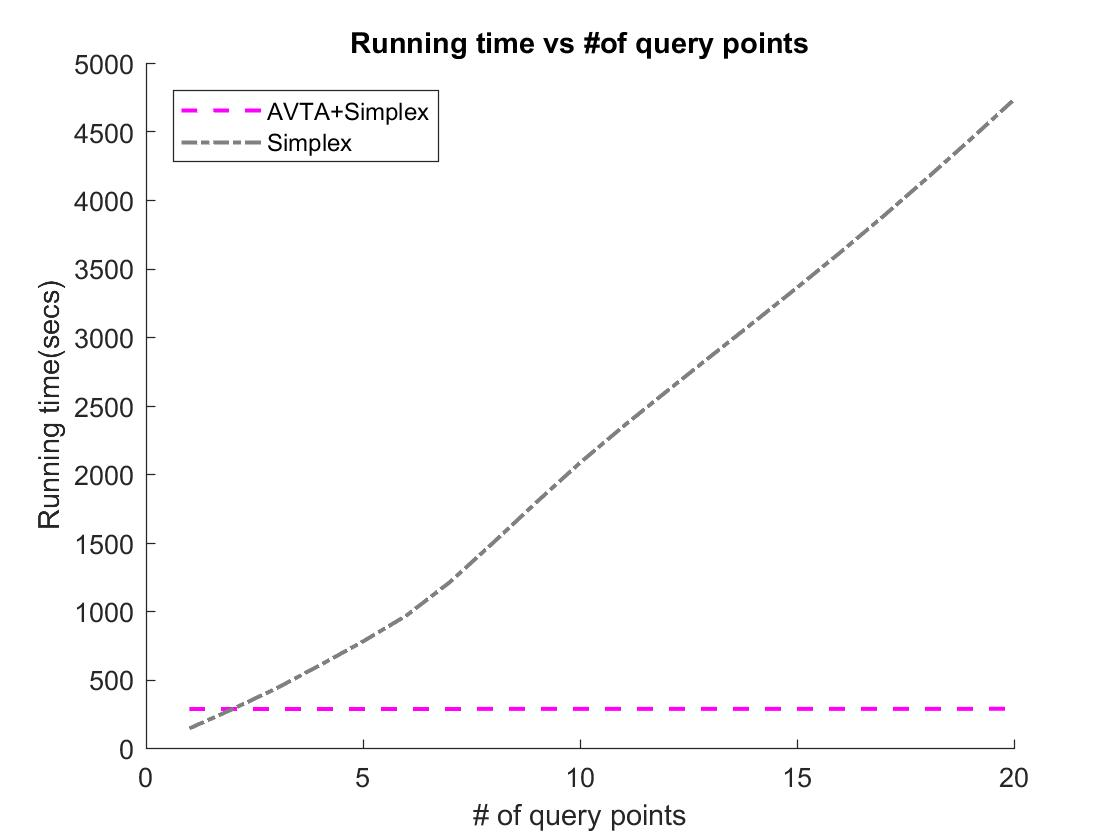
\includegraphics[width=0.95\textwidth]{nnsys.jpg}
				%\caption{(a)}
				
			\end{minipage}%
		}
		\caption{Running time for algorithms to find a feasible solution.}
		\label{fig:nnlsys-time}
	\end{figure}
	\noindent It can be observed from Figure~\ref{fig:nnlsys-time} and Table~\ref{tb:nnlsys time} that the running time of AVTA+Simplex doesn't have obvious increase while Simplex increases drastically. This suggests the potential applications of AVTA in dynamic linear feasibility problem.
	
	\subsubsection{Computing all vertices}
	\noindent\textbf{Compute vertices in high dimension} The convex hull vertices problem is to find all vertices of a set of points in $\mathbb{R}^m$. In general, computing exact vertices in dimension $d$ has worst complexity exponential in $d$  ~\cite{chazelle1993optimal}. However, given $conv(A)$ satisfying $\gamma$ robust assumption, $AVTA$ can compute the set of vertices efficiently. 
	
	\noindent
	In the experiment, we set $K=100$, $n=500$ and $m$ varying from $2 \sim 12$.~\footnote{ The maximum of dimension is $12$ in the experiment because of the explosion of running time of the \textbf{Quick hull} algorithm}.
	\noindent
	The computational results is shown in Table ~\ref{tb:avtaqhull}.  In high dimension $m \geq 9$, when $conv(S)$ is $\gamma$ robust for some $\gamma >0$, the \textbf{AVTA} algorithm successfully find all vertices of the convex hull efficiently while the \textbf{Quick hull} algorithm is stuck by its explosion of complexity in dimension $m$. 
	
	\begin{table}[!h]
		\centering
		\caption{Running time(secs)}
		\label{tb:avtaqhull}
		\scalebox{0.5}
		{
		\begin{tabular}{|l|l|l|l|l|l|}
			\hline
			dim & Qhull & AVTA  & dim & Qhull & AVTA  \\ \hline
			2   & 0.13      & 14.82 & 7   & 2.92      & 41.51 \\ \hline
			3   & 0.02      & 16.62 & 8   & 16.48     & 39.63 \\ \hline
			4   & 0.04      & 24.49 & 9   & 82.09     & 44.21 \\ \hline
			5   & 0.12      & 32.76 & 10  & 391.36    & 45.79 \\ \hline
			6   & 0.59      & 37.66 & 11  & 1479.51   & 51.19 \\ \hline
		\end{tabular}
	}
	\end{table}
		
	\begin{figure}[!h]
		\centering
		\scalebox{0.5}
		{
			\begin{minipage}[b]{0.95\linewidth}
				\centering
				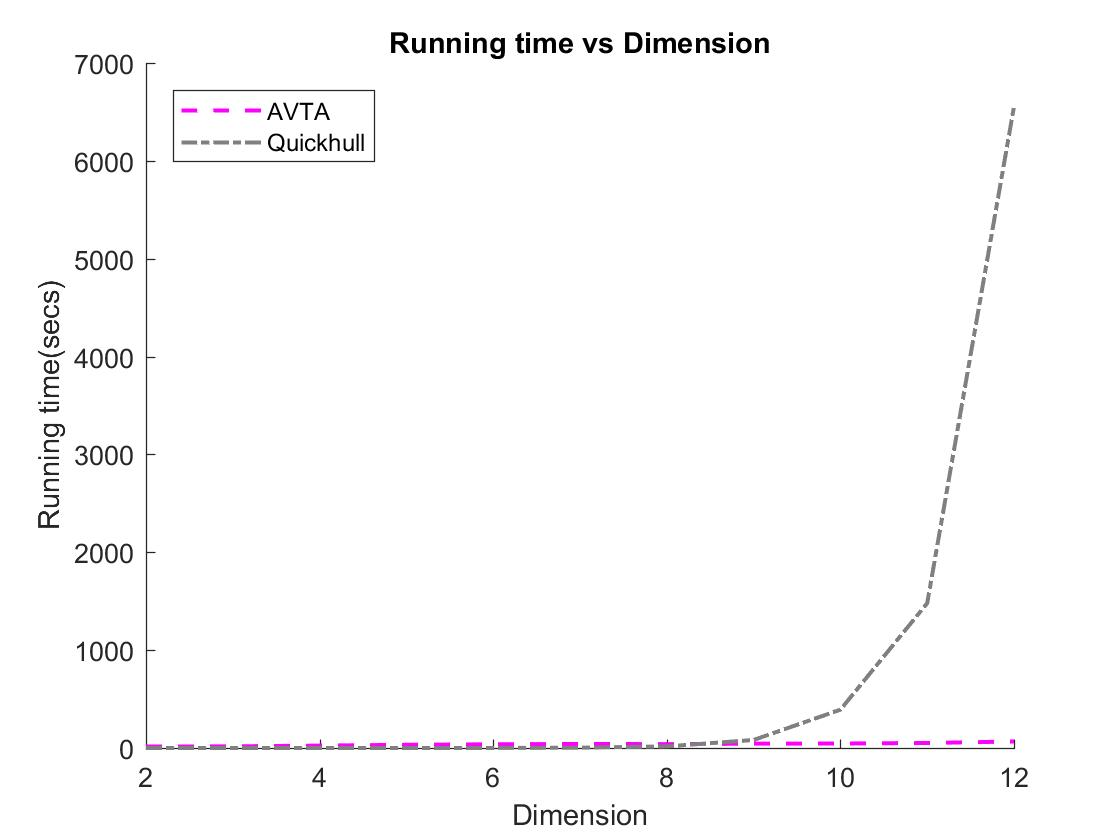
\includegraphics[width=0.95\textwidth]{tavsqhull.jpg}
				%\caption{(a)}
				\label{fig1}
			\end{minipage}%
		}
		\caption{Running time for algorithms to find all vertices.}
		\label{fig1}
	\end{figure}
	

	\noindent\textbf{Compute vertices with perturbation}:
	In this section, we compare \textbf{AVTA} with another robust algorithm \textbf{Fast Anchor Word}. 
	While the modified AVTA algorithm comes with theoretical guarantees, in certain cases the algorithm might output many more vertices, $K_\varepsilon$, than desired. Here we present a practical implementation that always outputs exactly $K$ vertices, provided $K$ is known. Notice that we want a fast way to detect good approximations to the original vertices of the set $S$ and prune out spurious points, i.e., additional vertices of the set $S_\varepsilon$. The key insight on top of the AVTA algorithm is the following: {\em If the perturbed set is randomly projected onto a lower dimensional space, it is more likely for an original vertex to still be a vertex than for a spurious vertex}. Using this insight the algorithm outlined below runs the modified AVTA algorithm over several random projections and outputs the set of points that appear as vertices in many random projections. 
	
	
	\begin{center}
		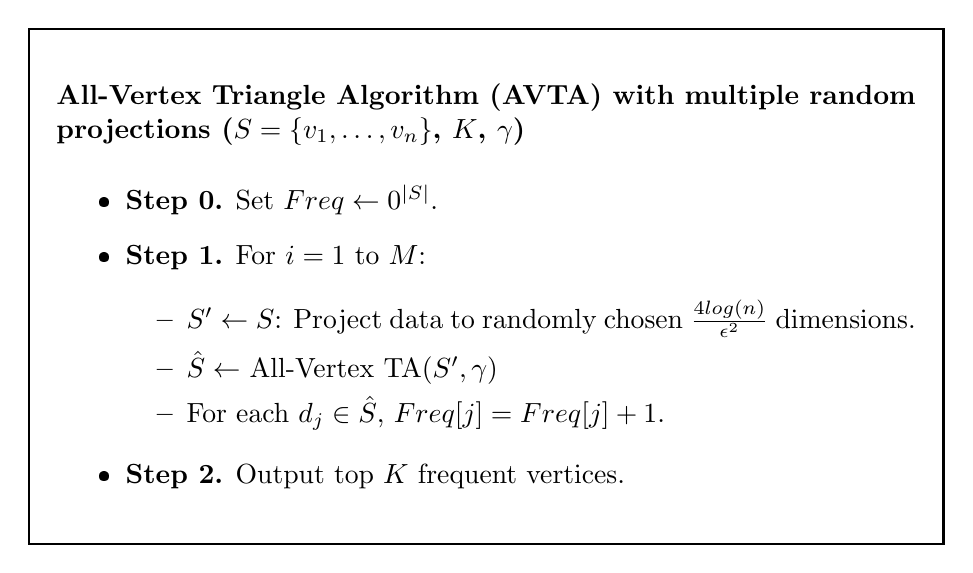
\begin{tikzpicture}
		%\begin{center}
		\node [mybox] (box){%
			\begin{minipage}{0.9\textwidth}
			{\bf  All-Vertex Triangle Algorithm (AVTA) with multiple random projections ($S=\{v_1, \dots, v_n\}$, $K$, $\gamma$)}\
			\vspace{.2cm}
			\begin{itemize}
			\item
			{\bf Step 0.} Set $Freq \leftarrow 0^{|S|}$.
			
			\item
			{\bf Step 1.} For $i=1$ to $M$:
			
			\begin{itemize}
			
			\item
			$S' \leftarrow S $: Project data to randomly chosen $\frac{4log(n)}{\epsilon^2}$ dimensions.
			
			\item 
			$\hat{S} \leftarrow $ All-Vertex TA$(S',\gamma)$
			
			\item 
			For each $d_j \in \hat{S}$, $Freq[j] = Freq[j] + 1$.
			
			
			\end{itemize}
			
			\item
			{\bf Step 2.} Output top $K$ frequent vertices.
			
			
			
			\end{itemize}
			\end{minipage}};
		\end{tikzpicture}
	\end{center}
	
	\noindent
	 We generate data according to a Gaussian distribution $\mathcal{N}(0,10) ^m$ with $m=100$. We generate $K=50$ such points and use them as the vertices of the convex hull. Given these vertices, $n=500$ interior points are generated as convex combination of the vertices, where the weights are generated  scaled i.i.d uniform distribution. We choose a Gaussian perturbation from $\mathcal{N}(0,\tau) ^m$ where $\tau$ varies from $0.3$ to $3$. 
	We  do an error analysis and evaluate the output of the algorithms by measuring the $l_2$ distance between true vertices and the convex hull of output vertices of the two algorithms.  More precisely, given a true vertex $v_i \in S$ and $\hat{S}$, the output of an algorithm, the error in recovering $v_i$ is defined to be $\min_{u\in conv(\hat{S})} \; ||u-v_i||_2.$ We add up all the errors to get the total accumulated error.
	\begin{table}[!h]
		\centering
		\caption{Recovery error (Simplex)}
		\label{tb:avta rec}
		\begin{tabular}{|l|l|l|}
			\hline
			variance & AVTA+Multiple Rp & Fast Anhor \\ \hline
			0.3      & 2.96             & 2.96       \\ \hline
			0.6      & 5.79             & 5.79       \\ \hline
			0.9      & 8.61             & 9.36       \\ \hline
			1.2      & 11.34            & 12.00      \\ \hline
			1.5      & 14.16            & 15.44      \\ \hline
			1.8      & 16.60            & 17.98      \\ \hline
			2.1      & 19.40            & 20.58      \\ \hline
			2.4      & 21.93            & 23.77      \\ \hline
			2.7      & 23.69            & 24.90      \\ \hline
			3        & 26.72            & 28.78      \\ \hline
		\end{tabular}
	\end{table}
	\begin{figure}[!h]
		\centering
		
		\begin{subfigure}{0.5\textwidth}
			\centering
			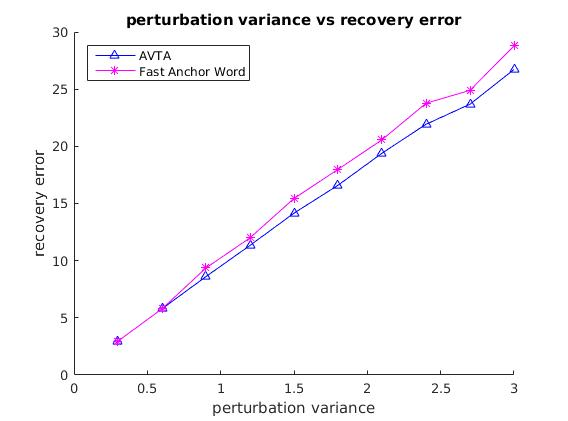
\includegraphics[width=0.5\textwidth]{AVTA_FAW_simplex}
			\caption{Simplex}
			\label{fig:avta rec}
		\end{subfigure}%
		\begin{subfigure}{0.5\textwidth}
			\centering
			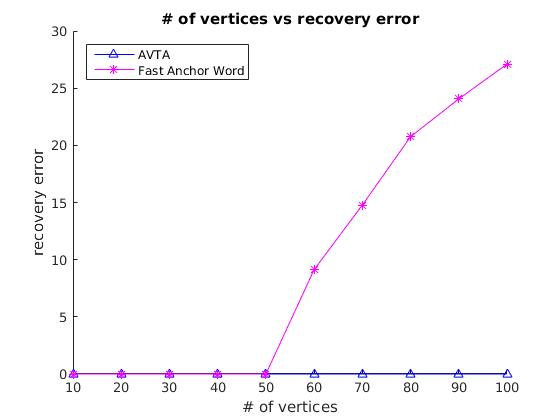
\includegraphics[width=0.5\textwidth]{AVTA_FAW_Polytope}
			\caption{General convex hull}
			\label{fig:synthetic-error-general}
		\end{subfigure}%
		\label{fig: AVTA vs FAW}
	\end{figure}\\
	\noindent
	Table~\ref{tb:avta rec} shows AVTA with multiple random projection has a better recovery error in the simplex case. 
	
	\noindent It can also be observed from Figure~\ref{fig:synthetic-error-general} that in general case, as number of vertices exceeds the number of dimensions, FAW fails to recover more vertices and its error explodes.  
	
	\subsection{Semi synthetic data and real data}
	
	\subsubsection{Topic modeling}
	We now show how AVTA can be used to solve the topic modeling in a variety of ways. We first look at how to solve the problem under the separability assumption.
	
	\noindent \textbf{AVTA in the presence of anchor words:}
	Arora et al.~\cite{arora2013practical} provide a practical algorithm for topic modeling with provable guarantees. Their algorithm works under the assumptions that the topic-word matrix is {\em separable}. In particular, they assume that corresponding to each topic $i$, there exists an {\em anchor word} $w_i$ that has a non zero probability of appearing only under topic $i$. Under this assumption, the algorithm of~\cite{arora2013practical} consists of two stages: a) find the anchor words, and b) use the anchor words to learn the topic word matrix. The problem of finding anchor words corresponds to finding the vertices of the convex hull of the word-word covariance matrix.  They propose an algorithm named {\em fast anchor words} in order to find the vertices. Since AVTA works in general setting, we can instead use AVTA to find the anchor words. Additionally, the fast anchor words algorithm needs to know the value of the number of anchor words, as an input. On the other hand, from the statements of Theorems~\ref{thm9} and\ref{thm13} it is easy to see that AVTA can work in a variety of settings when other properties of the data are known such as the robustness. We argue that robustness is a parameter that can be tuned in a better manner than trying different values of  the number of anchor words. In fact, one can artificially add random noise to the data and make it robust up to certain value. One can then run AVTA with the lower bound on robustness as input and let the algorithm automatically discover the number of anchor words. This is much more desirable in practical settings. Our first implementation of AVTA is named AVTA+RecoverL2 that uses AVTA to detect anchor words and then uses the anchor words to learn the topic word matrix using the approach from~\cite{arora2013practical}. AVTA is also theoretically superior than fast anchor words and achieves slightly better run times in the regime when the number of topics is $o(\log n)$, where $n$ is the number of words in the vocabulary. This is usually the case in most practical scenarios. 
	
	
	\noindent \textbf{AVTA in the absence of anchor words:} The presence of anchor words is a strong assumption that often does not hold in practice. Recently, the work of Bansal et al.~\cite{bansal2014provable} designed a new practical algorithm for topic models under the presence of catch words. Catch words for topic $i$ correspond to set $S_i$ such that it's total probability of appearing uunder topic $i$ is significantly higher than in any other topic. Their algorithm called TSVD recovers much better reconstruction of the topic-word matrix in terms of the $\ell_1$ error. They also assume that for each topic $i$, there are a few dominant documents that mostly contain words from topic $i$. The TSVD algorithm works in two stages. In stage 1, the (thresholded) word-document data matrix is projected onto a $K$-SVD space to compute a different embedding of the documents. Then, the documents are clustered into $K$ clusters. Under the assumptions mentioned above, one can show that the dominant documents for each topic will be clustered correctly. In stage 2, a simple post processing algorithm can approximate the topic-word matrix from the clustering.
	
	We improve on TSVD by asking the following question: {\it is $K$-SVD the right representation of the data?}. Our key insight is that if dominant documents are present in the topic, it is easy to show that most other documents will be approximated by a convex combination of the dominant topics. Furthermore, the coefficients in the convex combinations will provide a much more faithful low dimensional embedding of the data. Using this insight, we propose a new algorithm that runs AVTA on the data matrix to detect vertices and to approximate each point using a convex combination of the vertices. We then use the coefficient matrix as the new representation of the data that needs to be clustered. Once the clustering is obtained, the same post processing step from~\cite{bansal2014provable} can be used to recover the topic-word matrix. Our results show that the embedding produced by AVTA leads to much better reconstruction error than of that produced by TSVD. Furthermore, $K$-SVD is very sensitive to the presence of outliers in the data. In contrast, our new algorithm called AVTA+CatchWord is much more stable to noise in the data.
	\begin{center}
	
		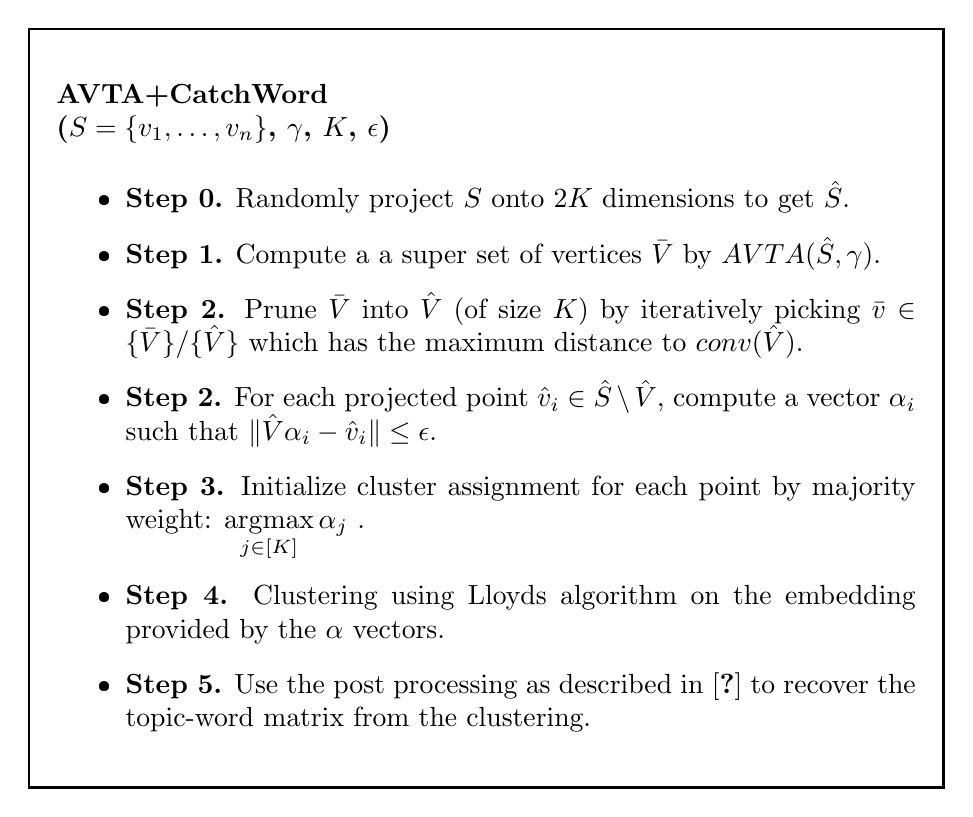
\begin{tikzpicture}
		%\begin{center}
		\node [mybox] (box){%
			\begin{minipage}{0.9\textwidth}
			{\bf  AVTA+CatchWord}\\
			{\bf ($S=\{v_1, \dots, v_n\}$, $\gamma$, $K$, $\epsilon$)}\
			\vspace{.2cm}
			\begin{itemize}
			\item
			{\bf Step 0.} Randomly project $S$ onto $2K$ dimensions to get $\hat{S}$.
			
			\item
			{\bf Step 1.} Compute a  a super set of vertices $\bar{V}$ by $AVTA(\hat{S}, \gamma)$.
			
			
			\item 
			{\bf Step 2.} Prune $\bar{V}$ into $\hat{V}$ (of size $K$) by iteratively picking $\bar{v} \in \{\bar{V}\}/\{\hat{V}\}$ which has the maximum distance to $conv(\hat{V})$.
			
			
			\item 
			{\bf Step 2.} For each projected point $\hat{v}_i \in \hat{S} \setminus \hat{V}$, compute a vector $\alpha_i$ such that $\|\hat{V} \alpha_i - \hat{v}_i\| \leq \epsilon$.
			
			\item
			{\bf Step 3.} Initialize cluster assignment for each point by majority weight: $ \argmax\limits_{j \in [K]} \alpha_j$	.
				
			\item 
			{\bf Step 4.} Clustering using Lloyds algorithm on the embedding provided by the $\alpha$ vectors.
			
			\item 
			{\bf Step 5.} Use the post processing as described in~\cite{bansal2014provable} to recover the topic-word matrix from the clustering.
			
			\end{itemize}
			\end{minipage}};
		\end{tikzpicture}
	\end{center}
	
	

	
	\noindent
	We compare our algorithms with the Fast Anchor + Recoverl2 algorithm of~\cite{arora2013practical} and the TSVD algorithm of~\cite{bansal2014provable} on two types of data sets: semi-synthetic data and real world data. 
	We next describe our methodology and empirical results in detail.
	
	
	
	\noindent \textbf{Semi Synthetic Data:} For Semi-Synthetic data set, we use similar methodology as in~\cite{arora2013practical}. We first train the model on real data set using Gibbs sampling with 1000 iterations. We choose $50$ as the number of topics which follows ~\cite{bansal2014provable,}.  Given the parameters learned from dataset, we generate documents with $\alpha$ set to be $0.01$. The average document length is 1000.  Then the reconstruction error is measured by the $l_1$ distance of bipartite matched pairs between  the true word-topic distribution and the  word-topic distribution~\cite{arora2013practical}. We then average the errors to compute the final mean error.
	
	\noindent \textbf{Real Data:} We use the \textbf{NIPS} data set with 1500 documents , and a pruned vocabulary of 2K words, and the NYTimes Corpus with sub sampled 30000 documents, and a pruned vocabulary of 5k words.~\footnote{\url{https://archive.ics.uci.edu/ml/datasets/bag+of+words}}. For our experiments on NMF we use the Swimmer data set~\cite{donoho2003does} that consists of $256$ swimmer figures with each a $32 \times 32$ binary pixel image. One can interpret each image as a document and pixels as a word in the document~\cite{ding2013topic}. All swimmers consist of $4$ limbs with each limb having $4$ different possible poses. One can then consider the different poses of limbs as the true underlying topics~\cite{donoho2003does}. We compare the algorithm proposed in~\cite{arora2012computing} with {AVTA+Recoverl2} on the swimmer data set.  Since the true underlying topics are known, we will plot the output of the algorithms and compare it with the underlying truth.
	
	
	\noindent \textbf{Implementation Details:} We compare 4 algorithms, {AVTA+CatchWord}, {TSVD}, the {Fast Anchor + Recoverl2} and the {AVTA+Recoverl2}. We implement our own version of Fast Anchor + Recoverl2 as described in~\cite{arora2013practical}. TSVD is implemented using the code provided by the authors in~\cite{bansal2014provable}. AVTA+Recoverl2 corresponds to using AVTA to detect anchor words from the word-word covariance matrix and then using the Recoverl2 procedure from~\cite{arora2013practical} to get the topic-word matrix. AVTA + CatchWord corresponds to finding the low dimensional embedding of each document in terms of the coefficient vector of its representation in the convex hull of the vertices. The next step is to cluster these points. In practice, one could use the Lloyd's algorithm for this step which could be sensitive to initialization.   To remedy this, we use similar heuristic as ~\cite{bansal2014provable} of the initialization step. We repeat \textbf{AVTA} for $3$ times and pick the set of vertices with highest quality. We set the number of output vertices $K=50$ which is the same as the number of topics. i.e. each vertex corresponds to a topic. We found that initializing by simply assigning clusters using neighborhoods of highest degree vertices works effectively. As a final step, we use the post processing step from~\cite{bansal2014provable} to recover the topic-word matrix from the clustering. 
	

	
	\noindent \textbf{Robustness:} We also generate perturbed version of the semi synthetic data. We generate a random matrix with i.i.d. entries uniformly distributed with different scales varying from $0.005-0.05$. We test all the algorithms with the document-word matrix added with the noise matrix.

	
	\noindent \textbf{Results on Semi Synthetic Data:}
	Figures~\ref{fig:semi-synthetic} and \ref{fig:semi-synthetic-noise} show the $\ell_1$ reconstruction of all the four algorithms under both clean and noisy versions of the semi synthetic data set. For topic $i$, let $A_i$ be the ground truth topic vector and $\hat{A}_i$ be the topic vector recovered by the algorithm. Then the $\ell_1$ error is defined as $\frac 1 K \sum_{i=1}^K \|A_i - \hat{A}_i\|_1$. The plots show that AVTA+CatchWord is consistently better than both TSVD and Fast Anchor + Recoverl2 and produces significantly more accurate topic vectors. In order to further test the robustness of out approach, we plot in Figure~\ref{fig:err_range} the range of the $\ell_1$ error obtained across multiple runs of the algorithms on the same data set. The range is defined to be the difference between the maximum and the minimum error recovered by the algorithm across different runs. We see that AVTA+CatchWord produces solutions that are much more stable to the effect of the noise as compared to other algorithms. Table~\ref{tb:runtime-4} shows the running time of the experiments of 4 algorithms. As can be seen, when using AVTA to learn topic models via the anchor words approach, our algorithm has comparable run time to Fast Anchor + Recoverl2. 
	\begin{figure}[!ht]
		\centering
		
		\begin{subfigure}{0.60\textwidth}
			\centering
			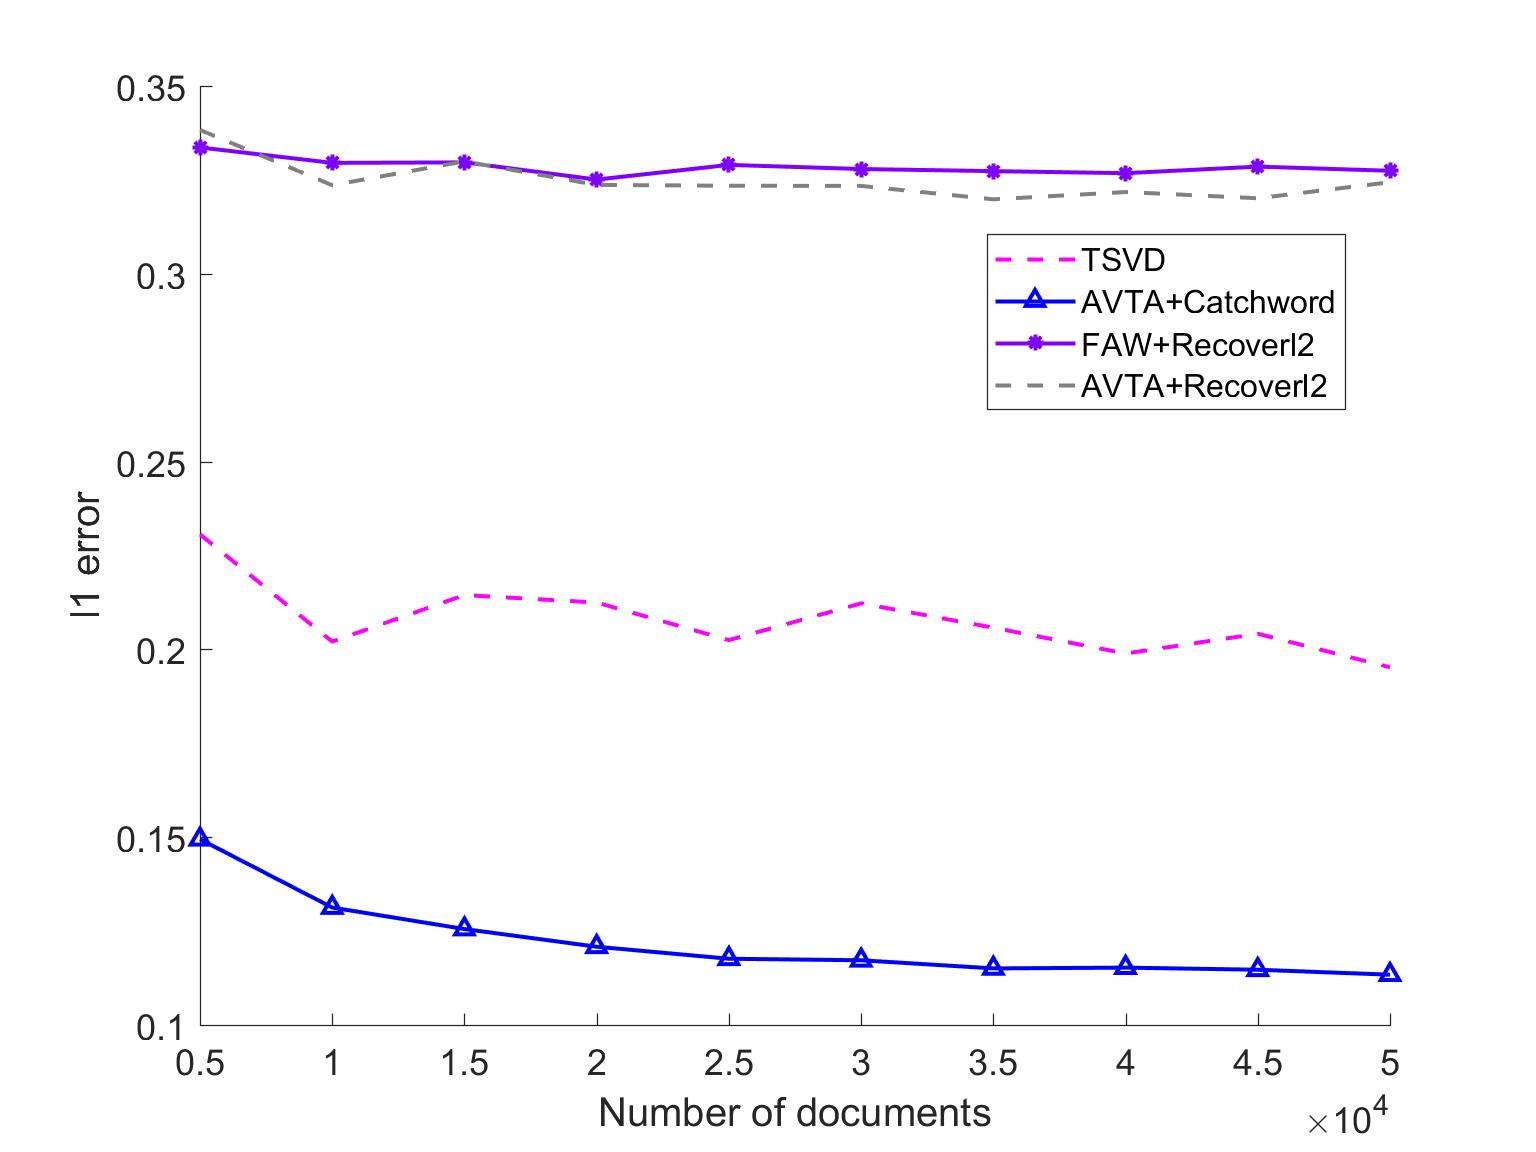
\includegraphics[width=0.3\textwidth]{Diff_number_of_doc}
			\caption{$\ell_1$ error in the semi-synthetic dataset ($K=50$).}
			\label{fig:semi-synthetic}
		\end{subfigure}%
		\begin{subfigure}{0.45\textwidth}
			\centering
			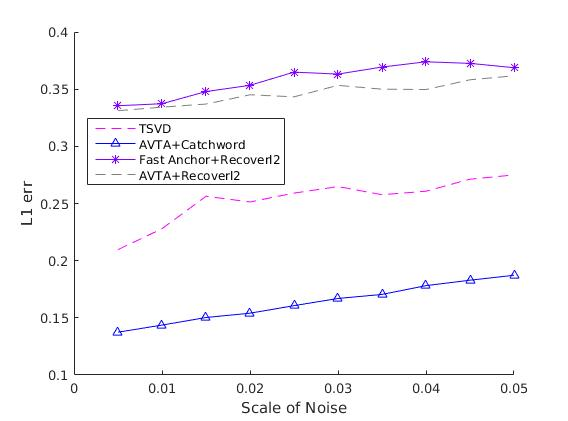
\includegraphics[width=0.4\textwidth]{err_diff_scale_noise}
			\caption{$\ell_1$ error in the perturbed semi-synthetic dataset ($K=50$).}
			\label{fig:semi-synthetic-noise}
		\end{subfigure}%
		
		\begin{subfigure}{0.55\textwidth}
			\centering
			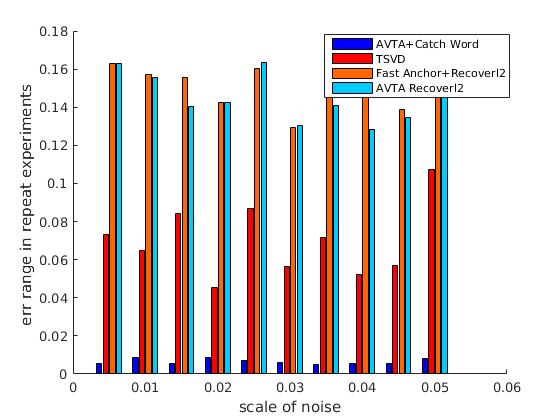
\includegraphics[width=0.3\textwidth]{range_diff_scale_noise.jpg}
			\caption{Range of the $\ell_1$ error over $10$ runs on the same data set.}
			\label{fig:err_range}
		\end{subfigure}%		
	\end{figure}
%	{\small
%		\begin{figure}[!h]
%			\centering
%			%\begin{subfigure}{0.5\textwidth}
%			%\centering
%			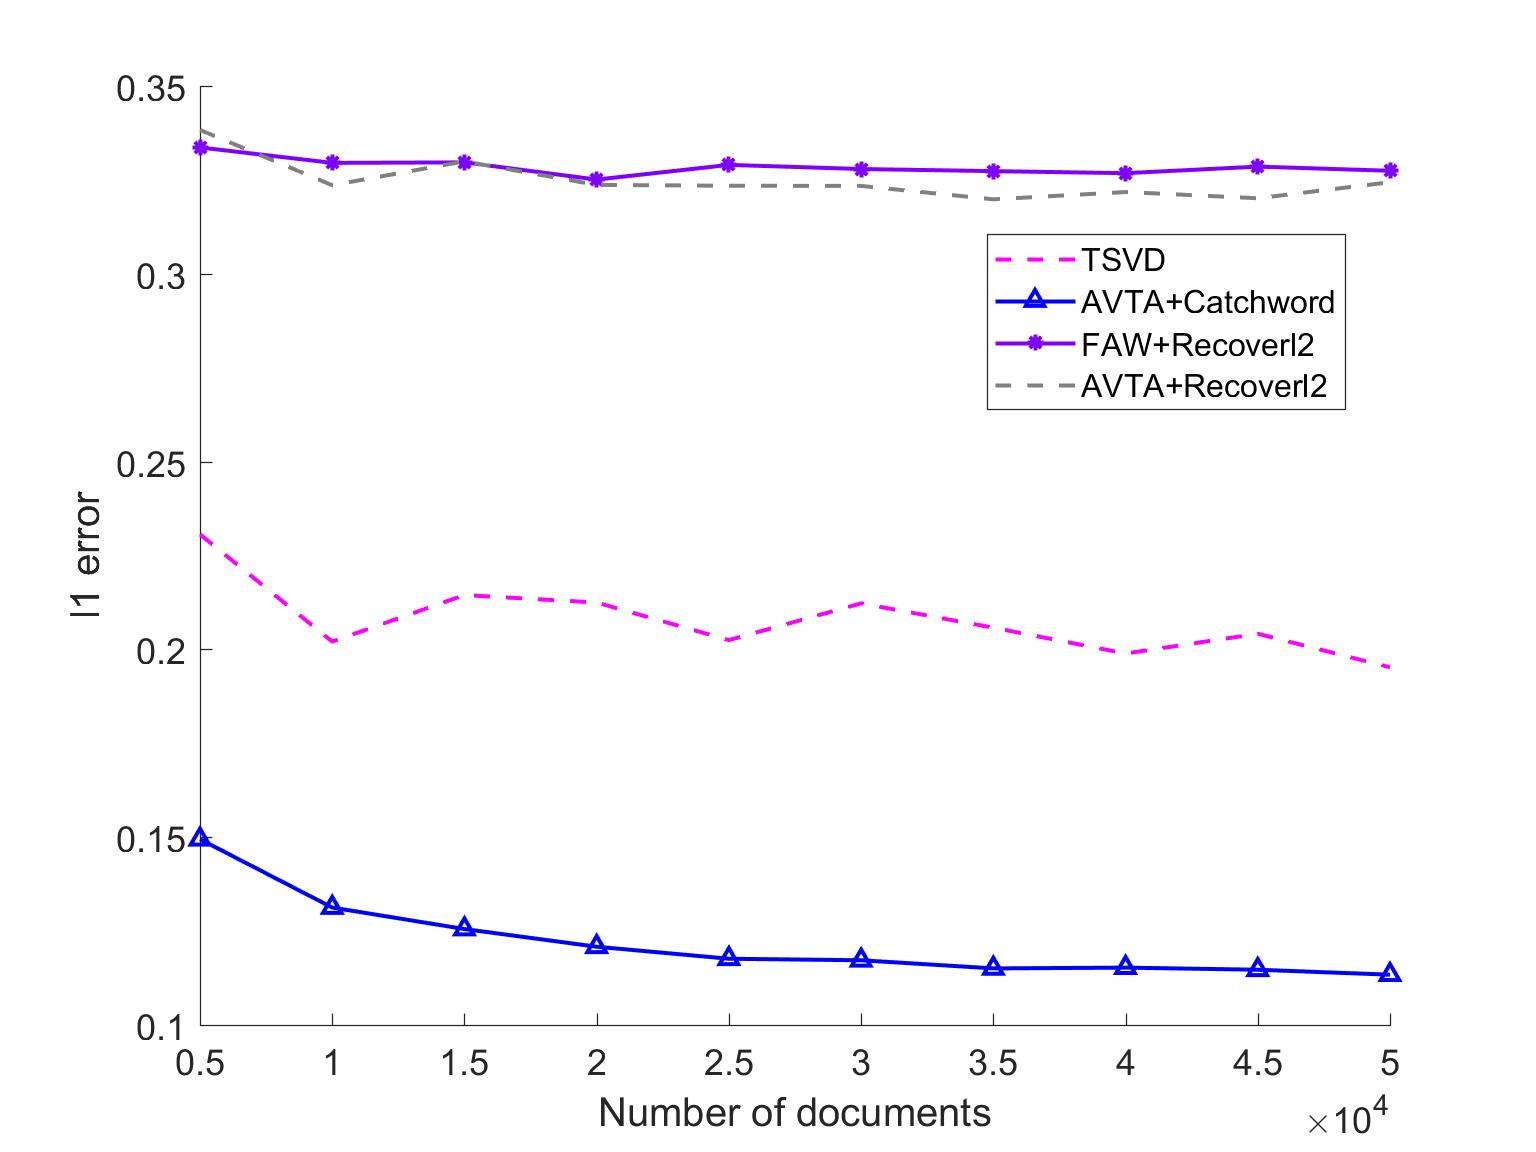
\includegraphics[width=0.5\textwidth]{Diff_number_of_doc}
%			\caption{$\ell_1$ error in the semi-synthetic dataset ($K=50$).}
%			\label{fig:semi-synthetic}
%			%\floatfoot{(a)}
%			%\end{subfigure}%
%		\end{figure}
%		\begin{figure}[!ht]
%			\centering
%			%\begin{subfigure}{0.5\textwidth}
%			%\centering
%			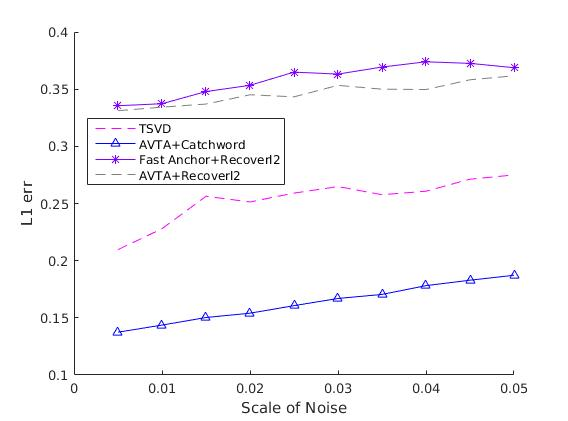
\includegraphics[width=0.5\textwidth]{err_diff_scale_noise}
%			\caption{$\ell_1$ error in the perturbed semi-synthetic dataset ($K=50$).}
%			\label{fig:semi-synthetic-noise}
%			%\floatfoot{(b)}
%			%\end{subfigure}\\
%		\end{figure}
%		\begin{figure}
%			%\begin{subfigure}{0.5\textwidth}
%			\centering
%			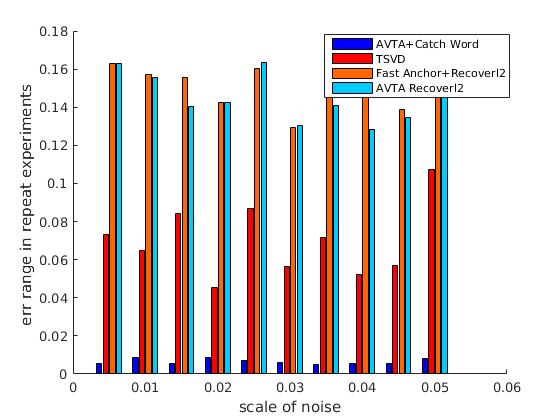
\includegraphics[width=0.5\textwidth]{range_diff_scale_noise.jpg}
%			\caption{Range of the $\ell_1$ error over $10$ runs on the same data set.}
%			\label{fig:err_range}
%		\end{figure}
%	}

	\begin{table}[!h]
		\centering
		\caption{Run time (in secs.) of algorithms on semi synthetic data}
		\label{tb:runtime-4}
		\begin{tabular}{|l|l|l|l|l|}
			\hline
			\begin{tabular}[c]{@{}l@{}}Num of\\   documents\end{tabular} & 5000 & 15000 & 30000 & 50000 \\ \hline
			Fast anchor+Recoverl2                                        & 5.49    & 6.00     & 10.30    & 13.60    \\ \hline
			AVTA+Recoverl2                                               & 7.82    & 7.68     & 12.84    & 16.40    \\ \hline
			TSVD                                                         & 17.02   & 43.27    & 81.24    & 112.80   \\ \hline
			AVTA+Catch Word                                              & 29.89   & 120.04   & 372.17   & 864.30   \\ \hline
		\end{tabular}
	\end{table}

	
	
	\noindent \textbf{Results on Real Data:}
	For the real world data set, as in prior works~\cite{arora2013practical, bansal2014provable}, we evaluate the coherence to measure topic quality~\cite{yao2009efficient}. Given a set of words $\mathcal{W}$ associated with a learned topic, the coherence is computed as:
	$Coherence(\mathcal{W})= \sum_{w_1,w_2 \in \mathcal{W}}  \log\frac{D(w_1,w_2)+\epsilon}{D(w_2)}$,
	where $D(w_1)$ and $D(w_1,w_2)$ are the number of documents where $w_1$ appears and $(w_1,w_2)$ appear together respectively~\cite{arora2013practical}, and $\varepsilon$ is set to $0.01$ to avoid $w_1,w_2$ that never co-occur~\cite{stevens2012exploring}. The total coherence is the sum of the coherence of each topic. In the NIPS dataset, $1000$ out of the $1500$ documents were selected as the training set to learn the word-topic distributions. The rest of the documents were used as the testing set. Table ~\ref{tb:real}  shows the topic coherence obtained by the algorithms. One can see that in both the approaches, either via anchor words or the clustering approach, AVTA based algorithms perform comparably to state of the art methods~\footnote{The topic coherence results for TSVD do not match the ones presented in~\cite{bansal2014provable} since in their experiments, the authors look at top 10 most frequent words in each topic. In our experiments we compute coherence for the top 5 most frequent words in each topic.}. The running  presented in ~\ref{tb:running time} shows AVTA based algorithm is efficient in real world data.
	
	
	
	\begin{table}[!h]
		\centering
		\caption{Topic coherence}
		\label{tb:real}
		\begin{tabular}{|l|l|l|l|l|}
			\hline
			& \tiny {Fast Anchor+RecoverL2} & \tiny { AVTA+RecoverL2} & TSVD     &  \tiny {AVTA+Catch Word} \\ \hline
			NIPS    & -15.8 $\pm 2.24$  & -16.04 $\pm 2.09$         & -16.86 $\pm 1.66$   & -18.65  $\pm 1.78$         \\ \hline
			NYTime  & -32.15  $\pm 2.7$                & -32.13    $\pm 2.43$     & -29.3933 $\pm 1.43$ & -30.13     $\pm 1.98$       \\ \hline
		\end{tabular}
	\end{table}
	
	\begin{table}[!h]
		\centering
		\caption{Running time on real data experiments}
		\label{tb:running time}
		\begin{tabular}{|l|l|l|l|l|}
			\hline
			&  \tiny {Fast Anchor+RecoverL2} &  \tiny {AVTA+RecoverL2} & TSVD  &  \tiny {AVTA+Catch Word} \\ \hline
			NY time & 26.05                 & 27.79          & 237.6 & 101.07          \\ \hline
			Nips    & 3.22                  & 4.41           & 56.58 & 22.78           \\ \hline
		\end{tabular}
	\end{table}
	
	\newpage
	\subsection{Non negative matrix factorization}
	\noindent \textbf{AVTA for NMF:} The work of~\cite{arora2012computing} showed that convex hull detection can be used to solve the non negative matrix factorization problem under the separability assumption. We show that by using the more general AVTA algorithm for solving the convex hull problem results in comparable performance guarantee.
	
	\noindent \textbf{Results on NMF:} The swimmer data set~\cite{donoho2003does} consists of $256$, $32 \times 32$ images and the task consists of inferring the underlying ``poses'' in a given image. In our experiments we use the original swimmer data set and also construct a noisy version by adding spurious poses. Let $\Omega(A)$ be a function that outputs a randomly chosen $32 \times 8$ block of an image. We generate a  'spurious pose' of size  $32\times 8$ by $\Omega(M_i)$ where $M_i$ is a randomly chosen swimmer image. Then we take another randomly chosen image $M_j$ and compute the corrupted image as $M'_j= M_j + c \cdot \Omega(M_i)$ where we simply set $c=0.1$. An illustration of the noise data set is shown in Figure~\ref{fig:Swimmer}. We compare the performance of AVTA on these data sets with the performance of the Separable NMF algorithm proposed in~\cite{arora2012computing}. Figures~\ref{fig:NMF swim} and ~\ref{fig:AVTA swim} show the output of the Separable NMF algorithm and that of our algorithm respectively on the noisy data set. Our approach produces competitive results as compared to the Separable NMF algorithm.
	
	\begin{figure}[!h]
		\centering
		%\begin{subfigure}{0.5\textwidth}
		%\centering
		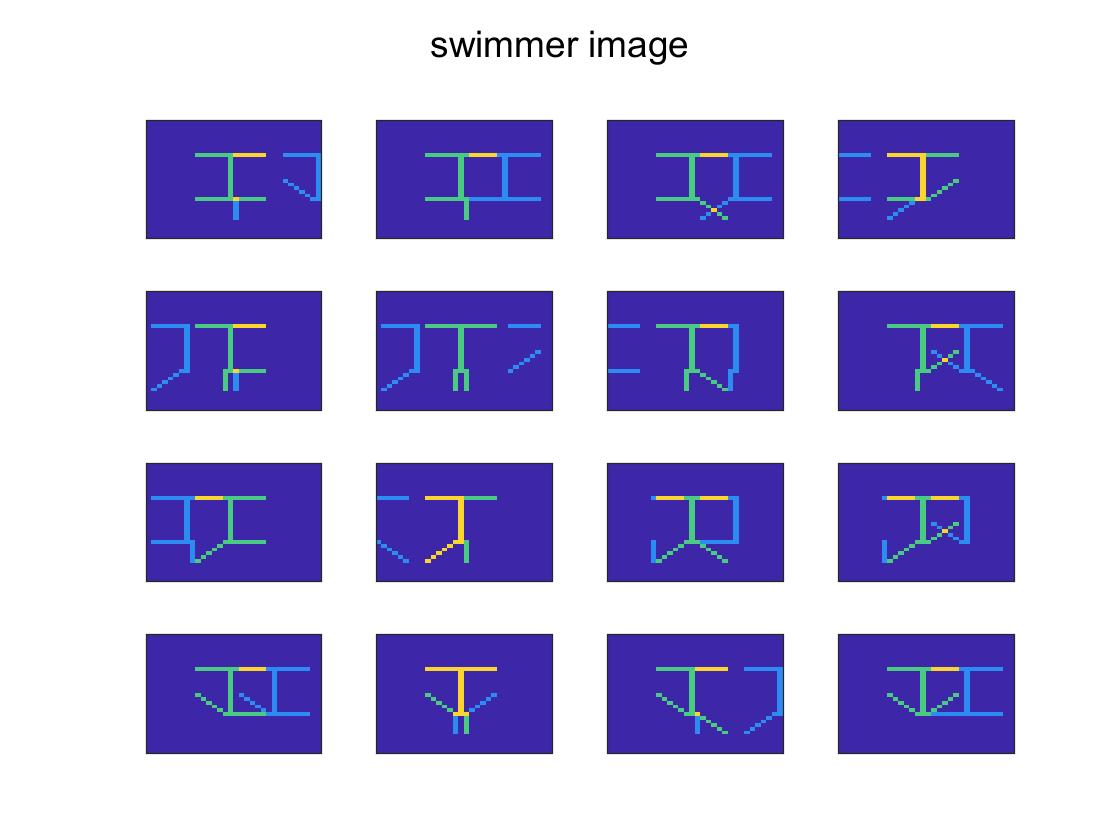
\includegraphics[width=0.5\textwidth]{swimmer_datasets.jpg}
		\caption{An example of spurious actions in swimmer images.}
		\label{fig:Swimmer}
		%\floatfoot{(b)}
	\end{figure}%\\
	\begin{figure}[!h]
		\centering
		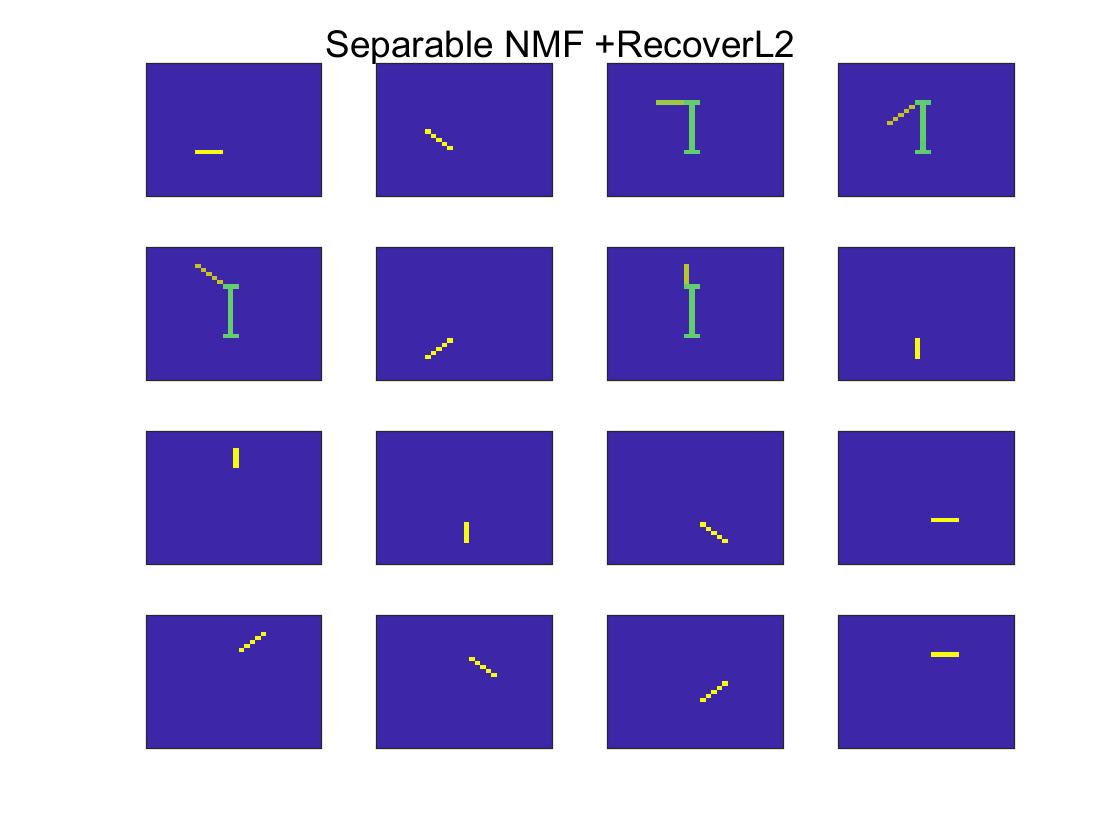
\includegraphics[width=0.5\textwidth]{swimmer_NMF.jpg}
		\caption{Output of {NMF +RecoverL2}}
		\label{fig:NMF swim}
		%\floatfoot{(a)}
	\end{figure}%
	\begin{figure}[!h]
		\centering
		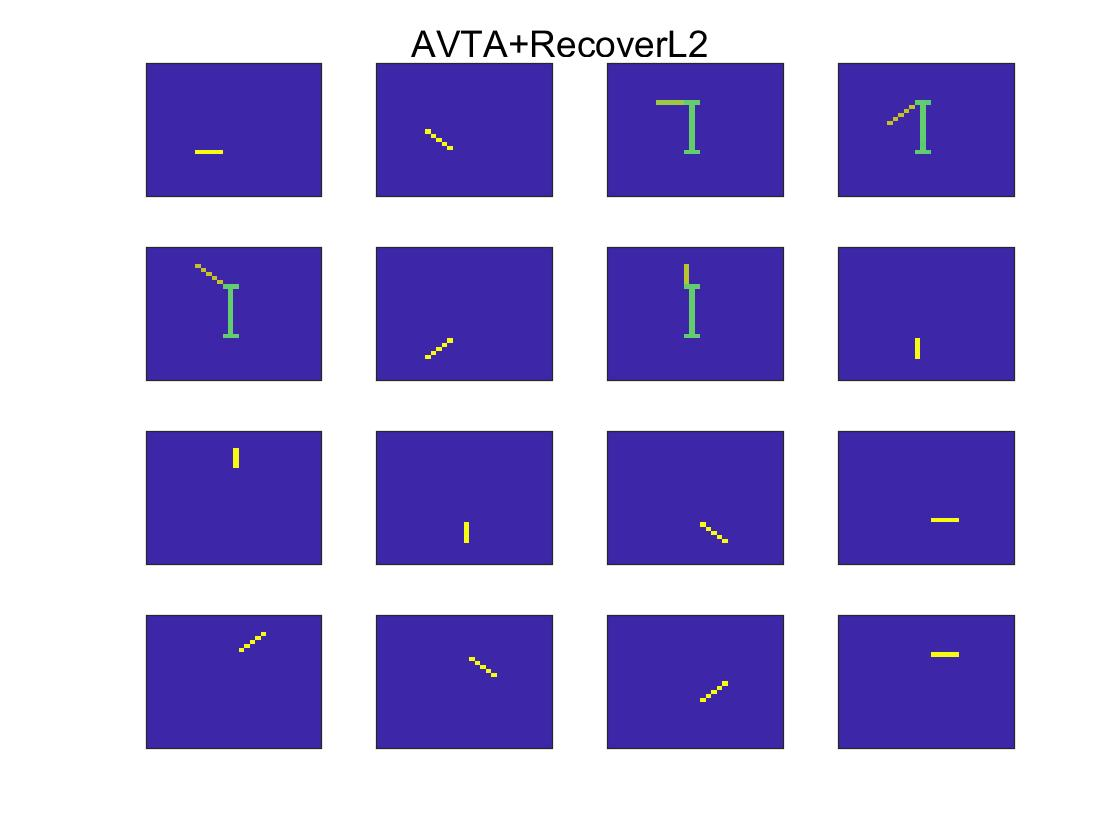
\includegraphics[width=0.5\textwidth]{swimmer_avta.jpg}
		\caption{Output of {AVTA +RecoverL2}}
		\label{fig:AVTA swim}
		%\floatfoot{(b)}
	\end{figure}

\newpage
\bibliographystyle{plain}
\bibliography{nips_2017}
\end{document}